% !TeX spellcheck = en_US
\chapter{Sim-to-Real Transfer}

\section{Introduction}
Check \textit{\citetitle{hofer2020perspectives}} \cite{hofer2020perspectives} to understand current limitations, directions, open questions, \etc.

For more application examples / experiments, check this \textit{mehhhhh} review: \textit{\citetitle{zhao2020sim}} \cite{zhao2020sim}

\section{Zero-shot Transfer}
\begin{itemize}
	\item Build a realistic simulator, or to have enough simulated experience
	\item Apply the model directly in real-world settings
\end{itemize}

\section{Domain Randomization}
\textit{Domain randomization} is the approach to vary the simulation settings, in hope that the model learns to generalize to real-world setting. In some sense, each roll-out is simply a sample from a certain distribution of simulation \ac{param}.
\begin{itemize}
	\item Can be divided into two kinds: \textit{visual randomization} and \textit{dynamics randomization}
	\item \citeausm{tobin2017domain} randomizes settings for pickup task
	\begin{itemize}
		\item Objects: number, shape, position and texture
		\item Camera: position, orientation, and field of view
		\begin{itemize}
			\item Position: random within a small fixed box $ (10\times5\times10cm) $ around initial point.
			\item The camera viewing angle: is offset by up to $ 0.1 rad $ from a fixed direction.
			\item The field of view is scaled by up to 5\% from the starting point.
		\end{itemize}	
		\item Lighting conditions: number, position, orientation, and specular characteristics.
	\end{itemize}
	\begin{figure}[hbt!]
		\centering
		\begin{subfigure}[b]{0.4\textwidth}
			\centering
			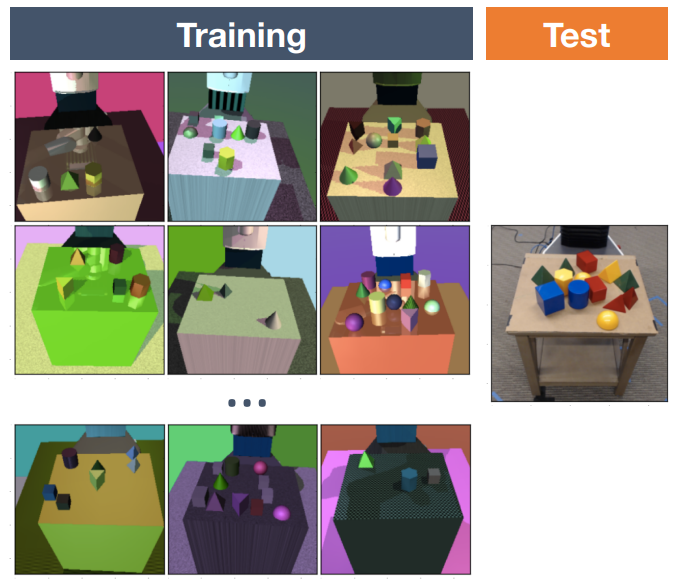
\includegraphics[width=\textwidth]{domain-randomization.png}
		\end{subfigure}
		\hfill
		\begin{subfigure}[b]{0.57\textwidth}
			\centering
			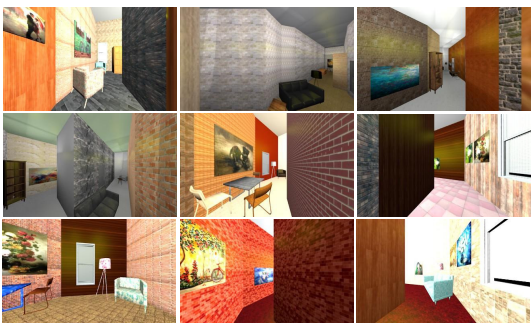
\includegraphics[width=\textwidth]{domain-randomization-1.png}
		\end{subfigure}
		\caption{Illustration of domain randomization \cite{sadeghi2016cad2rl, tobin2017domain}.}
		\label{fig:domain-randomization}
	\end{figure}	
	\item \citeausm{sadeghi2016cad2rl} randomize furniture, texture for drone's path planning problem.
\end{itemize}

\section{Adapting Simulation Randomization}
Domain randomization requires significant expertise and manual fine-tuning to design the distribution $ p(\xi) $ for simulation \ac{param}. In addition, overly wide distributions can hinder successful policy learning. The SimOpt approach adaptively optimize simulation \ac{param} with real-world experience. \cite{chebotar2019closing}

\section{Domain Adaptation}
\textit{Domain Adaptation} is the process that allow an \ac{AI} system trained in source domain to generalize to a target domain. In robotics, the source domain is the simulation and the target domain is the real world.
\begin{itemize}
	\item Labeled data is easily available from simulation / source domain
	\item Unlabeled data from real world / target domain can usually be collected, but labels are more difficult to obtain.
	\begin{itemize}
		\item \hlb{Unsupervised} domain adaptation: \hlr{no labels} in the target domain
		\item \hlb{Semi-supervised} domain adaptation: \hlr{fewer labels} in the target domain than in source domain
	\end{itemize}
	\item \textit{Pixel-level domain adaptation}: re-stylize images from the source domain to make them look like images from the target domain\\
	\note This is basically is neural style transfer in \ac{CV} with \ac{GAN}s\\
	Examples:
	\begin{itemize}
		\item \href{https://youtu.be/vDW8qvsBtmQ}{SimGAN} has \ac{GAN} and similarity loss \cite{shrivastava2017learning}
		\item \href{https://youtu.be/VhsTrWPvjcA}{PixelDA} adds task loss to the two above \cite{bousmalis2017unsupervised}
	\end{itemize}
	\item \textit{Feature-level domain adaptation}: focuses on learning domain-invariant features
	\begin{itemize}
		\item A mapping of fixed, pre-computed features between source and target domains \cite{sun2016return}
		\item DANN: A domain-invariant feature extractor with similarity loss (preferred method, using \ac{CNN}) \cite{ganin2016domain}
	\end{itemize}
\end{itemize}

Example:
\begin{itemize}
	\item Applying both pixel-level and feature-level domain adaptation: \citeaustitle{bousmalis2018using}
\end{itemize}

\section{Knowledge Distillation}
\textit{Policy distillation} is the process of extracting knowledge from a teacher network to a significantly smaller and more efficient student network, while maintaining a similarly expert level. The student is trained in a supervised manner with data generated by the teacher network.

\todo{DisCoRL, a modular, effective and scalable pipeline for continual learning}

\section{References}
\begin{itemize}
	\item Overview:
	\begin{itemize}
		\item \citeaustitle{hofer2020perspectives}
		\item \citeaustitle{zhao2020sim}
		\item Karol Arndt, Murtaza Hazara, Ali Ghadirzadeh, and Ville Kyrki. Meta reinforcement learning for sim-to-real domain adaptation. arXiv:1909.12906, 2019.
		\item Continual reinforcement learning deployed in real-life using policy distillation and sim2real transfer
	\end{itemize}
	\item Domain randomization:
	\begin{itemize}
		\item \citeaustitle{chebotar2019closing}
		\item \citeaustitle{tobin2017domain}
	\end{itemize}
	\item Domain adaptation:
	\begin{itemize}
		\item Pixel-level domain adaptation:
		\begin{itemize}
			\item \citeaustitle{shrivastava2017learning}
			\item \citeaustitle{bousmalis2017unsupervised}
		\end{itemize}
		\item Feature-level domain adaptation: \citeaustitle{ganin2016domain}
		\item Both: \citeaustitle{bousmalis2018using}
	\end{itemize}
	\item Knowledge distillation
\end{itemize}